\section{Introduction}
Une \emph{anomalie}, du grec $\ alpha \ nu \ omega \ mu \ alpha \ lambda \ iota \ alpha $, aspérité, irrégularité, non semblable (an-homalos), désigne un écart par rapport à une certaine norme, reflétant le comportement attendu.
On appelle \emph {anomalie} l'objet qui induit cet espace, l'observation qui s'écarte de la normalité.
%
Dans beaucoup de domaines, la situation suivante se présente: un expert cherche à prédire un phénomène sur la base d'observations antérieures. Le cas le plus fondamental est lorsque l'on veut prédire certaines caractéristiques binaires d'observations nouvelles, compte tenu des précédentes. Par exemple, on peut penser à un médecin voulant prédire si un nouveau patient présente ou non une certaine pathologie, en utilisant les données des patients précédents (comme l'âge, l'histoire, le sexe, la pression artérielle) associée à leur véritable \textbf{étiquette/label}: avoir ou non la pathologie en question). Ce cas est un exemple de \emph {classification binaire}, où le médecin cherche à trouver une règle pour \textbf {prédire} l'étiquette d'un nouveau patient (ce dernier étant caractérisé par son dossier médical, contenant toutes les mesures qui lui ont été faites). Cette règle est appelée un \emph{classifieur} et doit être construite, \emph{apprise}, sur des dossiers médicaux précédents. % (À savoir les enregistrements associés à leurs étiquettes).
Intuitivement, le classificateur prédit le même diagnostic pour des dossiers médicaux similaires, dans un sens qui doit être appris avec précision.

On peut distinguer deux cas. Si les étiquettes des patients antérieurs sont connues (porteur ou non de la pathologie), on dit que la tâche de classification est \textbf {supervisée}. Si les étiquettes de ces données d'entrainement sont inconnues, la classification est dite \textbf {non-supervisée}. Suivant notre exemple, le médecin doit trouver deux formes (ou cluster) distincts dans les données, correspondant aux deux étiquettes, "en bonne santé" - "malade", formes qui contiennent chacune des dossiers de patients similaires.

La détection d'anomalies survient lorsqu'une étiquette est fortement sous-représentée dans les données d'entrainement, par exemple si très peu de patients ont la pathologie dans les données d'entrainement.
Ainsi, la \textbf{détection d'anomalies supervisée} se résume à la classification supervisée de classes fortement déséquilibrées.
En ce qui concerne la \textbf {détection d'anomalie non supervisée} (également appelée simplement détection d'outliers), elle suppose généralement que la base de données a un modèle "normal" caché, et les anomalies sont des observations qui s'écartent de ce modèle. Le médecin veut trouver des dossiers médicaux qui s'écartent de la grande majorité de ceux de ses patients précédents.
%
Sa tâche est en quelque sorte simplifiée s'il sait que tous ses patients antérieurs sont en bonne santé: il est plus facile pour lui d'apprendre le modèle "normal", c'est-à-dire le dossier médical typique d'un patient en bonne santé, à confronté avec les dossiers médicaux de ses nouveaux patients. Ce cadre est celui de la \textbf {détection de nouveauté} -- également appelé classification à une classe ou détection d'anomalies semi-supervisées: les données d'entraînement ne contiennent que des instances normales.

Ce chapitre est organisé de la façon suivante.
Section~\ref{resume_fr:scoring_function}, la détection d'anomalie est formellement introduite, ainsi que la notion de fonction de score.
Deux critères sur la qualité d'une fonction de score sont ensuites présentés section \ref{resume_fr:scoring}.
La section ~\ref{resume_fr:extreme} se concentre sur la théorie des valeurs extrêmes (EVT) pour gagner en précision sur les régions extrêmes. Après avoir introduit la STDF (stable tail deviation function) representant la structure de dépendance des événements rares (Section ~\ref{resume_fr:stdf}), on montre que la théorie des extrêmes multivariées peut être utile pour produire des fonctions de score précise sur les régions de faible probabilité (Section ~\ref{resume_fr:sec:JMVA}).
La section ~\ref{resume_fr:sec:heuristic} regroupe deux contributions de nature heuristique portant d'une part sur l'évaluation / la sélection d'algorithmes de détection d'anomalies non supervisés (Section ~\ref{resume_fr:evaluation}) et d'autre part sur l'extension des forêts aléatoires à la classification à une classe (Section ~\ref{resume_fr:ocrf}). La section ~\ref{sec:impl} présente les contributions relatives à la librairie open-source scikit-learn. La section ~\ref{intro:concl} énumère les productions scientifiques et conclut.


\paragraph{Notations}

A travers ce document, $\mathbb{N}$ désigne l'ensemble des entiers naturels, $\mathbb{R}$ and $\mathbb{R}_+$ désigne respectivement les ensembles des nombres réels et celui des nombres réels positifs. Les ensembles  sont généralement écrit en lettre calligraphiques comme $\mathcal{G}$, et $|\mathcal{G}|$ désigne le nombre d'éléments dans $\mathcal{G}$. 

Ls vecteurs sont écrits en minuscules et en gras. Pour un vecteur $\mathbf{x}\in\mathbb{R}^d$ et $i\in \{1,\dots,d\}$, $x_i$ désigne la $i^{ème}$ composante de $\mathbf{x}$. Le produit scalaire entre deux vecteurs est noté $\innerp{\cdot,\cdot}$. $\|\cdot\|$ désigne une norme arbitraire (sur des vecteurs ou sur des matrices) et $\|\cdot\|_p$ la norme $L_p$.

Au long de cette thèse, $\PP[A]$ représente la probabilité de l'évènement $A\in \Omega$, l'espace de probabilité sous-jacent étant $(\Omega, \mathcal{F}, \PP)$. Nous utilisons la notation $\mathbb{E}[X]$ pour indiquer l'espérance de la variable aléatoire $X$. $X \overset{d}{=} Y$ signifie que $X$ et $Y$ sont égales en distribution et $X_n \overset{d}{\to} Y$ signifie que $(X_n)$ converge vers $Y$ en distribution. Nous utilisons souvent l'abréviation $\mb X_{1:n}$ pour désigner un échantillon \iid~$(\mb X_1,\ldots,\mb X_n)$.

Les notations sont résumées \tref{resume_fr:tab:notations}.

\begin{table}[!ht]
\begin{center}
\begin{footnotesize}
\begin{tabular}{lp{1cm}l}
\toprule
\textbf{Notation} && \textbf{Description}\\
\midrule
$\cdf$ && cumulative distribution function\\
$\rv$ && random variable\\
$\mathbb{R}$ && Set of real numbers\\
$\mathbb{R}_+$ && Set of nonnegative real numbers\\
$\mathbb{R}^d$ && Set of $d$-dimensional real-valued vectors\\
$\leb(\cdot)$ && Lebesgue measure on $\mathbb{R}$ or $\mathbb{R}^d$\\
$(\cdot)_+$ && positive part\\
$\vee$ && maximum operator\\
$\wedge$ && minimum operator\\
%$\mathbb{R}^{c\times d}$ && Set of $c\times d$ real-valued matrices\\
$\mathbb{N}$ && Set of natural numbers, i.e., $\{0,1,\dots\}$\\
%$\mathbb{S}^{d}_+$ && Cone of symmetric PSD $d\times d$ real-valued matrices\\
%$[k]$ && The set $\{1,2,\dots,k\}$\\
$\mathcal{G}$ && An arbitrary set\\
$|\mathcal{G}|$ && Number of elements in $\mathcal{G}$\\
%$\mathcal{G}^m$ && A set of $m$ elements from $\mathcal{S}$\\
%$\mathcal{X}$ && Input space\\
%$\mathcal{Y}$ && Output space\\
%$z=(x,y)\in\mathcal{X}\times\mathcal{Y}$ && An arbitrary labeled instance\\
$\mathbf{x}$ && An arbitrary vector\\
$\mb x < \mb y$ && component-wise vector comparison\\
$\mb m$ (for $m \in \rset$) && vector $(m,\ldots,m)$\\
$\mb x < m$ && means $\mb x < \mb m$\\
$x_j$ && The $j^{th}$ component of $\mathbf{x}$\\
$\delta_{\mb a}$ && Dirac mass at point $a \in \mathbb{R}^d$\\
$\lfloor \cdot \rfloor$ && integer part\\
$\innerp{\cdot,\cdot}$ && Inner product between vectors\\
%$[\cdot]_+$ && Hinge function\\
%$\mathbf{M}$ && An arbitrary matrix\\
%$\mathbf{I}$ && The identity matrix\\
%$M_{i,j}$ && Entry at row $i$ and column $j$ of matrix $\mathbf{M}$\\
$\|\cdot\|$ && An arbitrary norm\\
$\|\cdot\|_p$ && $L_p$ norm\\
%$\mathsf{x}$ && An arbitrary string\\
%$|\mathsf{x}|$ && Length of string $\mathsf{x}$\\
%$\mathsf{x_i},\mathsf{x_{i,j}}$ && $j^{th}$ symbol of $\mathsf{x}$ and $\mathsf{x_i}$\\
%$x\sim P$ && $x$ is drawn i.i.d. from probability distribution $P$\\
$A\Delta B$ && symmetric difference between sets $A$ and $B$ \\
$(\Omega, \mathcal{F}, \PP)$ && Underlying probability space\\
$\mathcal{S}$ && functions $s: \mathbb{R}^d \rightarrow \mathbb{R}_+ $ integrable \wrt~ Lebesgue measure (scoring functions)\\
$\overset{d}{\to}$ && Weak convergence of probability measures or \rv\\
$\mathbf{X}$ && A \rv~with values in $\mathbb{R}^d$\\
$\mathds{1}_{\mathcal{E}}$ && indicator function event $\mathcal{E}$\\
$Y_{(1)} \le \ldots\le Y_{(n)}$ && order statistics of $Y_1,\ldots,Y_n$\\
$\mb X_{1:n}$ && An \iid~sample $(\mb X_1,\ldots,\mb X_n)$\\
$\PP[\cdot]$ && Probability of event\\
$\EE[\cdot]$ && Expectation of random variable\\
$\Var[\cdot]$ && Variance of random variable\\

\bottomrule
\end{tabular}
\end{footnotesize}
\caption[Résumé des notations]{Summary of notation.}
\label{resume_fr:tab:notations}
\end{center}
\end{table}


\section{Détection d'anomalies, ranking d'anomalies et fonctions de scores}
\label{resume_fr:scoring_function}
D'un point de vue probabiliste, il existe différentes façons de modéliser les comportements normaux et anormaux, ce qui conduit à différentes méthodologies. Un modèle probabiliste naturel consiste à supposer deux processus de génération différents pour les données normales et anormales. Les données normales (resp. données anormales) sont générées selon une distribution $F$ (respectivement $G$). La distribution sous-jacente générale est alors un mélange de $F$ et $G$. L'objectif est de déterminer si une nouvelle observation $ \mb x $ a été générée à partir de $ F $ ou de $ G $. Le meilleur moyen de résoudre théoriquement ce problème est le test du rapport de vraisemblances, également appelé test de Neyman-Pearson. Si $ (\ud F / \ud G) (\mb x)> t $ avec un certain seuil $ t> 0 $, alors $ \mb x $ a été tiré de $ F $. Sinon, $ \mb x $ est tiré de $ G $. Cela revient à estimer l' \emph{ensemble de niveaux de densité} $ \{\mb x, (\ud F / \ud G) (\mb x)> t \} $ \citep{Scholkopf2001, Steinwart2005, Scott2006, VertVert}.
%
Comme les anomalies sont très rares, leur structure ne peut être observée dans les données, en particulier leur distribution $ G $.
%
Il est courant et commode de remplacer $ G $ dans le problème ci-dessus par la mesure de Lebesgue, de sorte qu'il se résume à l'estimation du niveau de densité de $ F $.
\citep{Scholkopf2001, Scott2006, VertVert}.

Cela revient à supposer que les anomalies sont uniformément réparties sur le support de la distribution normale. % \ Citep {Steinwart2005, Blanchard2010}.
Cette hypothèse est donc implicitement faite par une majorité d'ouvrages sur la détection de nouveauté.
%
Nous observons les données dans $ \rset ^ d $ à partir de la classe normale seulement, avec une distribution sous-jacente $ F $ et avec une densité $ f: \rset ^ d \to \rset $.
% Les données anormales sont présumées être dans la queue de $ F $.
Le but est d'identifier les caractéristiques de cette classe normale, telles que son support $ \{\mb x, f (\mb x)> 0 \} $ ou un certain niveau de densité fixé $ \{\mb x, f (\mb x )> T \} $ avec $ t> 0 $ près de $ 0 $.

La détection d'anomalies non supervisée est souvent considérée comme un problème de classification à une classe, où les données d'entraînement sont polluées par quelques éléments de la classe anormale: elle fait appel à des algorithmes à une classe \emph{robustes} aux anomalies.

%This way of modeling appeals for \emph{density level set estimation} analysis.

Une idée naturelle pour estimer les ensembles de niveaux de densité est de calculer une estimation de la densité et de considérer les ensembles de niveaux associés \citep{Tsybakov1997, Cuevas1997, Baillo2001, Baillo2003, Cadre2006, Rigollet2009, Mason2009}.
La densité est généralement estimée à l'aide d'un estimateur à noyau non paramétrique ou d'un estimateur de maximum de vraisemblance à partir d'une famille paramétrique de fonctions. Mais ces méthodes ne s'adaptent pas bien à la  grande dimension. D'une certaine manière, ces méthodes cherchent à capturer plus d'informations que nécessaire pour la tâche d'estimation d'ensemble de niveau, comme les propriétés locales de la densité qui sont inutiles pour cette tache. En effet, il s'avère que pour toute transformation croissante $ T $, les ensembles de niveaux de $ T \circ f $ sont exactement ceux de $ f $. Ainsi, il suffit d'estimer n'importe quel représentant de la classe des transformées croissantes de $ f $, pour obtenir des estimés d'ensemble de niveaux. Intuitivement, il suffit d'estimer le pré-ordre (le \emph {scoring}) induit par $ f $ sur $ \rset ^ d $. Définissons une \emph {fonction de score} comme toute fonction mesurable $ s: ~ \rset ^ d \to \rset _ + $ intégrable par rapport à la mesure de Lebesgue $ \leb (.) $ et $ \S $ l'espace De toutes les fonctions de score.
Toute fonction de score définit un pré-ordre sur $ \rset ^ d $ et donc un classement sur un ensemble de nouvelles observations. Ce classement peut être interprété comme un degré d'anormalité, plus $ s (x) $ est petit, plus $ x $ est normal. Notons que la plupart des algorithmes de détection d'anomalie renvoient plus qu'une étiquette binaire, normale / anormale. Ils renvoient une fonction de score, qui peut être convertie en prédiction binaire, généralement en imposant un seuil basé sur sa distribution statistique.


Supposons que nous voulons apprendre une fonction de score $ s $ dont le pré-ordre induit est "proche" de celui de $f$, ou de manière équivalente dont les ensembles de niveaux induits sont proches de ceux de $ f $. Le problème est de transformer cette notion de proximité en critère $ \crit $, les fonctions de score optimales $ s ^ * $ étant alors définies comme celles qui optimisent $ \crit $. Dans le cadre de l'estimation de la densité, la différence uniforme $ \| f - \hat f \| \\infty $ est un critère commun pour évaluer la qualité de l'estimation. Nous aimerions un critère similaire, mais qui est invariant par transformé croissante de $ \hat f $. En d'autres termes, le critère doit être défini de telle sorte que la collection d'ensemble de niveaux d'une fonction de score optimale $ s ^ * (x) $ coïncide avec celle liée à $ f $, et toute transformation croissante de la densité devrait être optimale au sens de $ \crit $.
Plus formellement, nous allons considérer $ \crit ^ {\Phi} (s) = \| \Phi (f) \| $ (au lieu de $ \| s - f \| $) 
avec $ \Phi: \mathbb {R} \to \mathbb {R} _ + $ vérifiant $ \Phi (T \circ s) = \Phi (s) $ pour toute fonction de score $ s $ et transformation croissante $ T $. Ici $ \Phi (s) $ désigne soit la courbe masse-volume $ MV_s $ de $ s $, soit sa courbe en excès-masse $ EM_s $, définies dans la section suivante.

Ce critère qui mesure la qualité d'une fonction de score est alors un outil pour construire / apprendre une bonne fonction de score.
Selon le paradigme de la minimisation du risque empirique, une fonction de score est construite en optimisant une version empirique $ \crit_n (s) $ du critère sur un ensemble adéquat de fonctions de score $ \S_0 $ de complexité contrôlée (par exemple une classe de dimension {\sc VC} finie).

La section suivante décrit deux critères fonctionnels au vue de la nature globale du problème, tout comme les courbes \roc (\emph{Receiver Operating Characteristic}) et PR (\emph {Précision-Rappel}, et qui sont admissibles par rapport aux exigences énumérées ci-dessus. Ces critères fonctionnels étendent en quelque sorte le concept de la courbe $ \roc $ au cadre non-supervisé.

\begin{remarque}{\bf Terminologie: détection d'anomalies, ranking d'anomalies.\\}
À proprement parler, les critères que nous recherchons sont des critères de \emph{ranking} d'anomalies, de la même manière que la courbe ROC est essentiellement un critère de \emph{ranking} bipartite.
%

En pratique comme mentionné ci-dessus, tous les algorithmes de détection d'anomalies sont candidats à la tâche de ranking d'anomalie. Ils produisent tous une fonction de score, même ceux qui traitent à l'origine du cadre de "classification des anomalies", c'est à dire cherchent à être optimal sur un seul ensemble de niveau ou pour un taux de faux positifs fixe.

Dans la littérature, la terminologie "détection d'anomalies" est largement utilisée, au lieu de la terminologie plus précise de "ranking d'anomalies". Par exemple, \cite{Liu2008} écrit "\emph{Le but de la détection d'anomalie est de fournir un ranking qui reflète le degré d'anomalie}".

Dans le cadre de ce travail, nous optons de même pour la convention que la détection d'anomalies se réfère au ranking d'anomalies: si les labels sont disponibles pour l'étape d'évaluation, l'objectif est de maximiser l'aire sous la courbe ROC. Si aucune donnée labelisée n'est disponible, l'objectif est de maximiser les critères non-supervisées définis dans la section suivante.

\end{remarque}


\section{M-estimation et critères de performance pour les fonctions de scores}
\label{resume_fr:scoring}
Cette section est un résumé du chapitre~\ref{aistat: chap}, qui est basé sur un travail publié en \cite{AISTAT15}. Nous fournissons un bref aperçu du critère de la courbe masse-volume introduit dans \cite{CLEM13}, qui est basé sur la notion d'ensembles de volume minimum. Nous exposons ensuite les principaux inconvénients de cette approche et proposons un autre critère, la courbe d'excès de masse.

\subsection{Ensembles à volume minimal}
\label{resume_fr:mv-set}

La notion d'ensemble à volume minimal (\cite{Polonik97, Einmahl1992}) a été introduite pour décrire des régions où une variable aléatoire multivarié $\mb X \in \rset^d$  se trouvent avec très grande ou très petite probabilité. Soit $\alpha \in (0,1)$, un ensemble à volume minimal $\Gamma^*_{\alpha}$ de masse au moins $\alpha $ est une solution du problème de minimisation sous contrainte

\begin{equation}\label{resume_fr:eq:MV}\min_{\Gamma~ \text{borelien}} ~\leb(\Gamma) \mbox{~tel que~} \mathbb{P}(\mb X \in \Gamma) \ge \alpha,
\end{equation}

le minimum étant pris sur tous les sous-ensembles mesurables $ \Gamma $ de $ \rset^d $.
On peut montrer que chaque niveau de densité est un ensemble à volume minimal pour une certaine masse et que la réciproque est vraie si la densité n'a pas de partie plate.
Dans le reste de cette section, on suppose que $F$ a une densité $ f(x) $ par rapport à la mesure de Lebesgue sur $ \rset^d $ satisfaisant les hypothèses suivantes:

\noindent $\mathbf{A_1}$ {\it La densité $f$ est bornée.}%, \textit{i.e.} $\vert \vert f(\mb X)\vert\vert_{\infty}<+\infty~.$}

\noindent $\mathbf{A_2}$ {\it La densité $f$ n'a pas de partie plate: $\forall c\geq 0$, $\mathbb{P}\{f(\mb X)=c\}=0~.$}

% Application of this concept includes in particular novelty/anomaly detection: for large values of $\alpha$, abnormal observations are those which belong to the complementary set $X\setminus\Omega^*_{\alpha}$
%  for each $\alpha \in (0,1)$ there exists a threshold value $t^*_{\alpha}$
% % \overset{def}{=}Q(f, \alpha)\geq 0
%  such that $\Omega^*_{\alpha}= \{ \mb x,f( \mb x) \ge t^*_{\alpha} \}$.
Sous les hypothèses précédentes, pour n'importe quel $\alpha\in (0,1)$, il existe un unique ensemble à volume minimal $\Gamma_\alpha^*$, dont la masse est equale à $\alpha$.
La fonction quantile (généralisée) est alors définie par:
$$
\forall \alpha\in (0,1),\;\; \lambda^*(\alpha) := \leb(\Gamma^*_{\alpha}).
$$

En outre, l'application $ \lambda^* $ est continue sur $(0,1)$ et uniformément continue sur $ [0,1- \epsilon] $ pour tout $ \epsilon \in (0,1) $ - quand le support de $ F $ est compacte, la continuité uniforme est valable sur l'intervalle fermé $[0,1] $.


Les estimés $ \widehat {\Gamma}^*_{\alpha} $ des ensembles à volume minimal sont construits en remplaçant la distribution de probabilité inconnue $ F $ par sa version empirique $ F_n = (1 / n) \sum_ {i = 1} ^ N \delta _ {\mb X_i} $ et en restraignant l'optimisation à une collection $ \mathcal{A} $ de sous-ensembles boréliens de $ \rset^d $. $ \mathcal {A} $ est supposée être assez riche pour inclure tous les ensembles de niveaux de densité, ou au moins des approximations raisonnables de ceux-ci.

Dans \cite{Polonik97}, les résultats limites sont prouvés pour le processus de quantile empirique généralisé $ \{\leb (\widehat {\Gamma}^*_{\alpha}) - \lambda^*(\alpha) \} $ (sous l'hypothèse en particulier que $ \mathcal{A} $ est une classe de Glivenko-Cantelli pour $ F $). Dans \cite {Scott2006}, il est proposé de remplacer le niveau $\alpha $ par $ \alpha- \phi_n $ où $ \phi_n $ joue le rôle d'un paramètre de tolérance (du même ordre que le supremum $\sup_{\Gamma\in \mathcal{A}}\vert F_n(\Gamma)-F(\Gamma) \vert$), la complexité de la classe $ \mathcal{A} $ étant contrôlée par la dimension {\sc VC}, afin d'établir des bornes. La version statistique du problème du volume minimal est alors

$$
\min_{\Gamma \in \mathcal{A}} \leb(\Gamma) \mbox{ subject to } F_n (\Gamma) \ge \alpha - \phi_n.
$$

L'ensemble $ \mathcal {A} $ de sous-ensembles boréliens de $ \rset^d $ offre dans l'idéal des avantages statistiques et computationnels, permettant une recherche rapide tout en étant suffisamment complexe pour capturer la géométrie des ensembles de niveaux de la densité - en d'autre termes, le "biais de modèle" $ \inf_ {\Gamma \in \mathcal{A}} \leb (\Gamma \Delta \Gamma^*_\alpha) $ doit être petit.

%Observe incidentally that the exact computation of the volume of a `complex' set may be challenging and estimates can be obtained by means of Monte-Carlo simulation.

\subsection{La courbe Masse-Volume}
\label{resume_fr:mv-curve}

Soit $s\in \mathcal{S}$ une fonction de score. Comme défini en \cite{CLEM13,CLEM14}, la courbe masse-volume de $s$ est le tracé de la fonction
\begin{align*}
MV_s : \alpha\in (0,1)\mapsto MV_s(\alpha) = \lambda_s \circ \alpha_s^{-1}(\alpha),
\end{align*}
où $ H ^ {- 1} $ désigne la pseudo-inverse de n'importe quelle cdf $H: \mathbb {R} \rightarrow (0,1) $ et où $ \alpha_s $ et $ \lambda_s $ sont définis par
\begin{equation}
\begin{aligned}
\label{resume_fr:eq:alpha_beta}
&\alpha_s(t):= \mathbb{P}(s(\mb X) \ge t), \\
&\lambda_s(t):=\leb(\{\mb x \in \rset^d, s(\mb x) \ge t\})~.
\end{aligned}
\end{equation}
%

Ceci induit un ordre partiel sur l'ensemble de toutes les fonctions de score: $ s $ est préférée à $s'$ si $MV_{s}(\alpha) \le MV_{s'}(\alpha)$ pour tout $\alpha \in (0,1) $. De plus, la courbe masse-volume reste inchangée lors de l'application d'une transformation croissante sur $ s $.
On peut prouver que $ MV ^ * (\alpha) \leq MV_s (\alpha) $ pour tout $ \alpha \in (0,1) $ et toute fonction de score $ s $, où $ MV ^ * (\alpha ) $ est la valeur optimale du problème de minimisation sous contrainte~\eqref{resume_fr:eq:MV}, à savoir

%
\begin{align}
\label{resume_fr:def:MV}
MV^*(\alpha)= \leb(\Gamma_\alpha^*)=\min_{\Gamma~ mes.} ~\leb(\Gamma) \mbox{~subject to~} \mathbb{P}(\mb X \in \Gamma) \ge \alpha~.
\end{align}
%
Sous les hypothèses $ \mathbf {A_1} $ et $ \mathbf {A_2} $, on peut montrer que la courbe $ MV^ * $ est bien une courbe masse volume, associée à (toute transformation croissante de) la densité $f$ à savoir: $ MV ^ * = MV_f $.

L'objectif est alors de construire une fonction de score $ \hat s $ en fonction des données d'entraînement $ \mb X_1, ... \mb X_n $ telle que $ MV_{\hat s} $ soit minimale partout, 
c'est-à-dire minimisant $\|MV_{\hat s}-MV^*\|_{\infty}:=\sup_{\alpha\in[0,1]}\vert MV_{\hat s}(\alpha)-MV^*(\alpha)\vert$.

\begin{figure}[h]
\centering
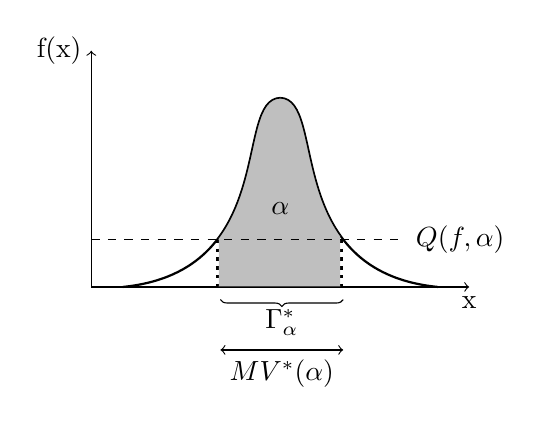
\begin{tikzpicture}[scale=2]

\draw[->](7.8,0)--(10.2,0) node[below]{x};
\draw[->](7.8,0)--(7.8,1.5) node[left]{f(x)}; 
\draw [thick] (8,0) ..controls +(1,0.1) and +(-0.3,-0.01).. (9,1.2);
\draw [thick] (9,1.2) ..controls +(0.3,-0.01) and +(-1,0.1).. (10,0);

\draw[dotted,very thick](8.60,0.3)--(8.60,0) node[right]{};
\draw[dotted,very thick](9.39,0.3)--(9.39,0) node[right]{};

%\draw (8,0.3)--(10,0.3)--(10,1.5)--(8,1.5)--(8,0.3); dessine 4 segments correspondant au 4 points

%hachurage :
\begin{scope} 
\clip (8.61,0)--(9.38,0)--(9.38,1.5)--(8.61,1.5)--(8.61,0) ; %tout ce qui est dans begin{scope} se limitera au rectangle

\path[draw,fill=lightgray] (8,0) ..controls +(1,0.1) and +(-0.3,-0.01).. (9,1.2)--
(9,1.2) ..controls +(0.3,-0.01) and +(-1,0.1).. (10,0)--
(8,0)--(10,0) --cycle;
\end{scope}

\draw[dashed](7.8,0.3)--(9.8,0.3) node[right]{$Q(f,\alpha)$};

%accolade :
\draw[decorate,decoration={brace}]
(9.4,-0.08)--(8.62,-0.08) node[below,pos=0.5] {$\Gamma_\alpha^*$};

\draw[<->]
(9.4,-0.4)--(8.62,-0.4) node[below,pos=0.5] {$MV^*(\alpha)$};



\draw (9,0.5) node[thick]{ $\alpha$} ;
%\draw (8.8,-0.8) node[thick]{Figure 1: MV curve} ;
\end{tikzpicture}
\caption{Masse-Volume au niveau $\alpha$}
\label{resume_fr:MVcurve}
\end{figure}

Pour ce faire, il faut d'abord estimer une collection d'ensembles à volume minimal relatifs aux masses cibles $ 0 <\alpha_1 <\ldots <\alpha_K <1 $ formant une subdivision de $ (0,1) $ sur la base des données d'entrainement afin de définir $s=\sum_k \mathds{1}_{\{x\in \hat \Gamma_{\alpha_k}^*\}}$. L'analyse se fait sous des hypothèses adéquates (relatives à $ \mathcal {G} $, au périmètre de $ \Gamma ^ * _ {\alpha_k} $ et au pas de la subdivision en particulier) et pour un choix approprié de $ K = K_n $.
Cependant, par construction, les vitesse d'apprentissage sont plutôt lentes (de l'ordre $ n ^ {- 1/4} $) et ne peuvent pas être établies lorsque le support n'est pas borné.

Les quatre principaux inconvénients de ce critère de courbe masse-volume sont les suivants.

\begin{itemize}
\item[\textbf{1)}] Lorsqu'il est utilisé comme critère de performance, la mesure de Lebesgue d'ensembles pouvant être très complexes doit être calculée.
\item[\textbf{2)}] Lorsqu'il est utilisé comme critère de performance, il n'existe pas de méthode directe pour comparer les courbes MV puisque la zone sous la courbe est potentiellement infinie.
\item[\textbf{3)}] Lorsqu'il est utilisé comme critère d'apprentissage, il produit des ensembles de niveaux qui ne sont pas nécessairement imbriqués, puis des fonctions de notation imprécises.
\item[\textbf{4)}] Lorsqu'il est utilisé comme un critère d'apprentissage, les taux d'apprentissage sont plutôt lents (de l'ordre $ n ^ {- 1/4} $), et ne peuvent pas être établis dans le cas d'un support non borné.
\end{itemize}




Dans la section suivante, et comme contribution de cette thèse, un autre critère fonctionnel est proposé, obtenu en échangeant objectif et contrainte dans \eqref{resume_fr:eq:MV}. Les inconvénients du critère de la courbe masse-volume sont résolus à l'exception du premier, et l'on montre que l'optimisation d'une version discrète empirique de cette mesure de performance donne des fonctions de score avec des taux de convergence de l'ordre $ \mathcal {O} _ {\mathbb {P}} (1 / \sqrt {n}) $. En outre, les résultats peuvent être étendus à la situation où le support de la distribution $ F $ n'est pas compact. De plus, lorsqu'on relaxe l'hypothèse faite dans l'analyse de la courbe masse-volume que tous les vrais ensembles de niveaux sont inclus dans notre classe de minimisation $ \mathcal {A} $, un contrôle du biais du modèle est établi. Enfin, nous déduisons des propriétés théoriques (non statistiques) vérifiées par ce critère, ce qui corrobore sa qualité de métrique sur les ensembles de niveaux contenus dans les fonctions de score.


\subsection{Le critère d'excès de masse}
\label{resume_fr:em-curve}
%The contribution summarized here has been published in~\cite{AISTAT15}.
Nous proposons un autre critère de performance qui s'appuie sur la notion de \textit {d'excès de masse} et d' \textit{ensemble de contours de densité}, comme introduits dans la contribution \cite{Polonik95}. L'idée principale est de considérer une formulation lagrangienne d'un problème de minimisation sous contrainte, obtenu en échangeant la contrainte et l'objectif dans \eqref{resume_fr:eq: MV}: pour $ t> 0 $,

\begin{equation}
\label{resume_fr:solomeg}
\max_{\Omega~ \text{borelien}}  \left\{ \mathbb{P}(\mb X \in \Omega) - t \leb(\Omega) \right\}.
\end{equation}
On désigne par $ \Omega ^ * _ t $ une solution de ce problème. Cette formulation offre certains avantages à la fois computationnels et théoriques: en laissant (une version discrétisée) du multiplicateur lagrangien $ t $ augmenter de $ 0 $ à l'infini, on peut facilement obtenir des solutions à la contrepartie empirique de \eqref{resume_fr:solomeg } formant une suite \textit {imbriquée} d'ensembles, évitant ainsi une dégradation du taux de convergence due à la transformation des solutions empiriques pour forcer la monotonie.

%
%\subsubsection{Theoretical study}
La \textbf{courbe d'excès de masse optimale} d'une distribution de probabilité  $F$ est définie comme le graphe de la fonction
$$t>0~~\mapsto~~ EM^*(t):=\max_{\Omega\text{ borelian} } \{ {\mathbb{P}} (\mb X\in \Omega)-t\leb(\Omega) \}.$$ 
Avec les notations précédente, nous avons: $EM^*(t)=\mathbb{P}(\mb X \in \Omega_t^*)-t \leb(\Omega_t^*)$ pour tout $t>0$.
Remarquons que $EM^*(t) = 0$ pour tout $t>\|f\|_\infty:=\sup_{x\in \rset^d}\vert f(x)\vert$. 
%
  La \textbf{courbe d'excès de masse} de $s\in\mathcal{S}$ par rapport à la distribution de probabilité $F$ d'une variable aléatoire $\mb X$ est le graphe de la fonction
\begin{equation}
\label{resume_fr:EM}
EM_s : t \in [0, \infty[ \mapsto \sup_{A \in \{(\Omega_{s,l})_{l>0}\}}\{ {\mathbb{P}}(\mb X \in A) - t \leb(A)\},
\end{equation}
où $\Omega_{s,t}=\{ x \in \rset^d, s(x) \ge t \}$ pour tout $t>0$.

On peut également écrire $ EM_s $ en termes de $ \lambda_s $ et $ \alpha_s $ définis en \eqref{resume_fr:eq:alpha_beta}, $EM_s(t)= \sup_{u>0}~ \alpha_s(u) -t \lambda_s(u) $. Enfin, sous l'hypothèse $ \mathbf {A_1} $, nous avons $ EM_s (t) = 0 $ pour tout $t> \|f\|_\infty$.

%
\begin{center}
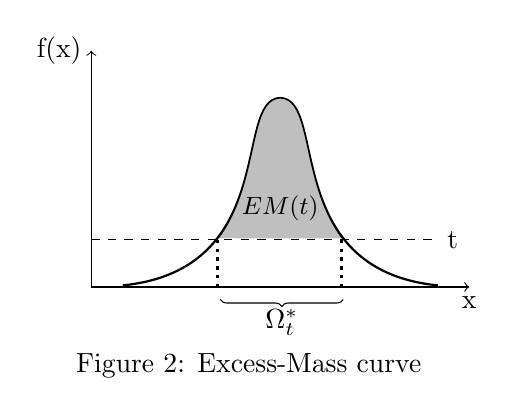
\begin{tikzpicture}[scale=2]
\draw[->](7.8,0)--(10.2,0) node[below]{x};
\draw[->](7.8,0)--(7.8,1.5) node[left]{f(x)}; 
\draw [thick] (8,0.01) ..controls +(1,0.1) and +(-0.3,-0.01).. (9,1.2);
\draw [thick] (9,1.2) ..controls +(0.3,-0.01) and +(-1,0.1).. (10,0.01);
\draw[dashed](7.8,0.3)--(10,0.3) node[right]{t};
\draw[dotted,very thick](8.60,0.3)--(8.60,0) node[right]{};
\draw[dotted,very thick](9.39,0.3)--(9.39,0) node[right]{};
%
%\draw (8,0.3)--(10,0.3)--(10,1.5)--(8,1.5)--(8,0.3); dessine 4 segments correspondant au 4 points
%
%hachurage :
\begin{scope} 
\clip (8,0.31)--(10,0.308)--(10,1.5)--(8,1.5)--(8,0.308) ; %tout ce qui est dans begin{scope} se limitera au rectangle (8,0.3)--(10,0.3)--(10,1.5)--(8,1.5)--(8,0.3)
\path[draw,fill=lightgray] (8,0) ..controls +(1,0.1) and +(-0.3,-0.01).. (9,1.2)--
(9,1.2) ..controls +(0.3,-0.01) and +(-1,0.1).. (10,0)--
(8,0.3)--(10,0.3) --cycle;
\end{scope}

%accolade :
\draw[decorate,decoration={brace}]
(9.4,-0.08)--(8.62,-0.08) node[below,pos=0.5] {$\Omega_t^*$};

\draw (9,0.5) node[]{\small $EM(t)$} ;
\draw (8.8,-0.5) node[thick]{Figure 2: Excess-Mass curve} ;
\end{tikzpicture}
\label{resume_fr:EMcurve}
\end{center}
%
\noindent
La maximisation de $ EM_s $ peut être vue comme trouver une collection de sous-ensembles $ (\Omega ^ * _ t) _ {t> 0} $ avec une masse maximale lorsqu'ils sont pénalisés par leur volume de façon linéaire. Une fonction de score optimale est alors n'importe quel $ s \in \S $ admettant $ \Omega^*_t $ 's comme ensembles de niveau, par exemple une fonction de score de la forme
\begin{align*}
%\label{score_cont}
s(x)=\int_{t=0}^{+\infty} \mathds{1}_{x\in \Omega^*_t}a(t)dt,\end{align*}
avec $a(t)>0$ (notons que $s(x)=f(x)$ pour $a \equiv 1$).
%
La fonction $EM_s$ est décroissante sur $(0,+\infty)$, à valeurs dans $[0,1]$ et satisfait, $EM_s(t) \le EM^*(t)$ pour tout $t\geq 0$. 
De plusn, pour $t \ge 0$ et pour n'importe quel $\epsilon > 0$, nous avons 
\begin{align*}
%\label{i}
\inf_{u>0} \epsilon \leb (\{ s >u\}\Delta_\epsilon \{f>t\}) ~\le~ EM^*(t)-EM_s(t) ~\le~ \|f\|_\infty \inf_{u>0} \leb (\{ s >u\}\Delta\{f>t\})
\end{align*}
avec $\{ s >u\}\Delta_\epsilon \{f>t\} ~:=~~ \{f>t+\epsilon\} \setminus \{ s >u\} ~~~\bigsqcup~~~ \{ s >u\} \setminus \{f>t-\epsilon\}$. Ainsi la quantité $EM^*(t)-EM_s(t)$ mesure avec quelle qualité les ensembles de niveaux de $s$ peuvent-il approchés ceux de la densité sous-jacente.
Sous des hypothèse raisonnables, (voir \cite{AISTAT15}, Prop.1), nous avons aussi pour $\epsilon >0$, 
\begin{align*}
%\label{ii}
\sup_{t\in[\epsilon ,\|f\|_\infty]}|EM^*(t)-EM_s(t)| ~~\le~~  C \inf_{T  \in \mathcal{T}} \|f-T\circ s\|_\infty
\end{align*}

où l'infimum est pris sur l'ensemble $ \mathcal {T} $ de toutes les transformations croissantes mesurables $T: \mathbb {R} _ + \rightarrow \mathbb {R} _ + $.
Les inégalités précédentes révèlent que $ \| EM ^ * - EM_s \| _ \infty $ peut être interprété comme une pseudo distance, soit entre les ensembles de niveaux de $ s $ et ceux de la densité sous-jacente $ f $, soit entre les pré-ordres induits par $ s $ et $ f $.

Le concept de la courbe EM fournit un moyen simple de comparer les fonctions de score, mais l'optimisation d'un tel critère fonctionnel est loin d'être simple. Comme proposé dans \cite {CLEM13} pour le critère MV, l'optimisation est faite sur une certaine classe de fonctions de score, que nous espérons assez riche pour fournir une bonne approximation (biais de modèle petit) tout en étant assez simple pour contrôler le taux de convergence. Nous considérons ici les fonctions de score de la forme

\begin{align*}
%\label{score}
s_N(x):= \sum_{k=1}^N a_k \mathds{1}_{x \in \hat{\Omega}_{t_k} }~, ~~~\text{with ~~~} \hat{\Omega}_{t_k}  \in \mathcal{G}
\end{align*}
où $\mathcal{G}$ est une class VC de sous-ensembles de $\rset^d$.
Nous choisissons de manière arbitraire $a_k:= (t_k-t_{k+1})$ de tel sorte que les $\hat{\Omega}_{t_k}$ correspondent exactement aux ensembles de niveau $t_k$, $\{s \ge t_k\}$. Ensuite, la maximisation du critère fonctionnel d'excès de masse s'effectue en résolvant de manière séquentielle, pour $k=1,\ldots,N$,
\begin{align*}
\hat \Omega_{t_k} \in \argmax_{\Omega \in \mathcal{G}} \frac{1}{n}\sum_{i=1}^n\mathds{1}_{X_i \in \Omega}~-~t_k \leb(\Omega).
\end{align*}

Les solution $ \hat \Omega_ {t_k} $ de ces problèmes d'optimisation peuvent toujours être choisie de manière à être imbriquée (contrairement au problème d'optimisation analogue pour le critère masse-volume). En d'autres termes, une contrainte d'inclusion peut être incorporée dans le problème d'optimisation précédent, sans affecter la qualité de la solution obtenue.Dans le cadre du critère masse-volume, des hypothèses sont faites stipulant que le support de la distribution doit être compact et que la classe VC $ \mathcal {G} $ doit contenir les vrais ensembles de niveaux de la densité. Ici, nous relaxons ces hypothèses, la première en choisissant des niveaux adaptatifs $ t_k $, et la seconde en dérivant une étude de biais. Ceci est détaillé chapitre~\ref{aistat: chap}.



\section{Précision sur les régions extrêmes}
\label{resume_fr:extreme}
\subsection{Analyse du point de vue de la théorie des valeurs extrêmes par l'estimation de la STDF}
\label{resume_fr:stdf}
Cette section est un résumé du chapitre~\ref{colt}, qui est basé sur le travail publié dans \cite{COLT15}.

Rappelons que les fonctions de score sont construites en approchant les ensembles de niveaux de densité / ensembles à volume minimal de la densité "normale" sous-jacente. Comme nous l'avons mentionné précédemment, dans le cadre de la détection d'anomalie, nous souhaitons être précis sur des ensembles de niveaux correspondant à des quantiles élevés, à savoir avec un niveau $ t $ près de $ 0 $ -- ou de manière équivalente, être précis sur des ensembles à volume minimal avec une contrainte de masse $ \alpha $ proche de $ 1 $.

%
Dans le cas univarié, supposons que nous voulons considérer le quantile $ (1-p) ^ {th} $ de la distribution $ F $ d'une variable aléatoire $ X $, pour une probabilité donnée de dépassement $ p $, c'est-à-dire
 $x_p = \inf\{x \in \mathbb{R},~ \mathbb{P}(X > x) \le p\}$. 
Pour les valeurs modérées de $ p $, une contrepartie empirique naturelle est
 $x_{p,n} = \inf\{x \in \mathbb{R},~ 1/n \sum_{i=1}^n \mathds{1}_{X_i > x}\le p\}$.
Cependant, si $ p $ est très petit, l'échantillon fini $ X_1, \ldots, X_n $ ne contient pas suffisamment d'informations $ x_ {p, n} $ devient inutile.
%
Ce problème devient dans le cas multivarié celui d'estimer des ensembles de niveaux de densité avec un niveau très faible ou de manière equivalente celui d'estimer les fonctions de score associées à ces ensembles de niveaux.
%
La théorie des valeurs extrêmes traite spécialement de ces problèmes, aussi bien dans le cadre unidimensionnel que multidimensionnel.
%


\paragraph{Preliminaries.}
La théorie de la valeur extrême (\textsc {EVT}) développe des modèles pour apprendre l'insolite plutôt que l'habituel. Ces modèles sont largement utilisés dans les domaines de la gestion des risques comme celui de la finance, de l'assurance, des télécommunications ou des sciences de l'environnement. Une application majeure de la \textsc{EVT} est de fournir une évaluation raisonnable de la probabilité d'occurrence d'événements rares.

Pour illustrer ce point, supposons que nous voulons gérer le risque d'un portefeuille contenant $ d $ actifs différents, $ \mb X = (X_1, \ldots, X_d) $. Un but assez général est alors d'évaluer la probabilité d'événements du type
 $\{X_1 \ge x_1 \text{ or }  \dotsc \text{ or } X_d\ge x_d \}$, 
pour des seuils multivariés grands $\mb x=(x_1,\ldots,x_d)$. Dans des conditions pas trop strictes sur la régularité de la distribution $ \mb X $, la \textsc {EVT} montre que pour des seuils suffisamment importants,
\[
\P\{X_1 \ge x_1 \text{ or }  \dotsc \text{ or }
X_d\ge x_d \} \simeq 
l(p_1,\ldots,p_d), 
\] 
où $ l $ est la STDF \emph{stable tail dependence function} et où les $ p_j $  sont les probabilités de dépassement marginal, $ p_j = \P (X_j \ge x_j) $. La fonction $ l $ caractérise la \emph {dépendance} entre les extrêmes. La distribution \emph {jointe} (sur des seuils importants) peut donc être récupérée à partir de la connaissance des distributions marginales avec la \textsc {stdf} $ l $. Dans la pratique, $ l $ peut être tirée de données "modérément extrêmes", typiquement les $ k $ `plus grandes 'parmi un échantillon de taille $ n $, avec $ k \ll n $.

L'estimation des $ p_j $ peut s'effectuer suivant un chemin bien pavé: dans le cas univarié, la \textsc {EVT} consiste essentiellement à modéliser la distribution des maxima (\emph {resp.} la queue supérieure) en tant qu'élément des familles paramétriques de Gumbel, Fréchet ou Weibull (\emph {resp.} par une distribution de Pareto généralisée).

Par contre, dans le cas multivarié, il n'y a pas de paramétrisation fini-dimensionnelle de la structure de dépendance.
Ce dernier étant caractérisé par le \textsc {stdf}, l'estimation de ce fonctionnel est l'un des principaux problèmes de la \textsc {EVT} multivariée. Les propriétés asymptotiques de la contrepartie empirique de la \textsc {stdf} ont été largement étudiées, voir \cite {Huangphd, Drees98, Embrechts2000, dHF06} pour le cas bivarié et \cite {Qi97, Einmahl2012} pour le cas général multivarié sous hypothèses de fluidité.

Cependant, aucune borne n'existe sur l'estimation non-asymptotique. La contribution résumée dans la section suivante et publiée dans \cite{COLT15} dérive de telles bornes non asymptotiques. Nos résultats ne nécessitent aucune hypothèse autre que l'existence de la \textsc {stdf}.


\paragraph{Apprentissage de la structure de dépendance des événements rares.}
Les inégalités de VC classiques visent à bourner la déviation des quantités empiriques par rapport aux quantités théoriques sur des classes d'ensemble relativement simples, appelées classes VC. Assez souvent, ces classes recouvrent tout le support de la distribution sous-jacente. Cependant, lorsqu'il s'agit d'événements rares, il est intéressant d'avoir de telles bornes sur une classe d'ensembles qui ne couvre qu'une région de faible probabilité et contient donc (très) peu d'observations. Cela donne des bornes plus fines, puisque seules les différences entre de très petites quantités sont impliquées dans l'analyse. Le point de départ est l'inégalité VC énoncée ci-dessous et prouvée dans le chapitre~\ref {colt}.

\begin{theorem}
\label{resume_fr:thm-princ} 
Soit $\mathbf{X}_1,\ldots,\mathbf{X}_n$ des réalisations \iid~d'une variable aléatoire $\mathbf{X}$, $\mathcal{A}$  une classe VC de VC-dimension $V_{\mathcal{A}}$. 

Considerons la classe $\mathbb{A} = \cup_{A \in \mathcal{A}} A$, et posons $p = \mathbb{P}(\mathbf{X} \in \mathbb{A})$. 
Alors il existe une constante absolue $ C $ de sorte que pour tout $ 0 <\delta <1 $, avec probabilité au moins $ 1- \delta $,
\begin{align*}
\sup_{A \in \mathcal{A}} \left| \mathbb{P} \big[\mathbf{X} \in A\big] - \frac{1}{n} \sum_{i=1}^n \mathds{1}_{\mathbf{X}_i \in A}  \right| ~~\le~~ C \bigg[ \sqrt{p}\sqrt{\frac{V_{\mathcal{A}}}{n} \log{\frac{1}{\delta}}} + \frac{1}{n} \log{\frac{1}{\delta}} \bigg]~.
\end{align*}
\end{theorem}

L'idée principale est la suivante. L'estimateur empirique de la {\sc stdf} est basé sur la mesure empirique des régions "extrêmes", qui sont touchées seulement avec une faible probabilité. Il suffit donc de borner les déviations maximales sur ces régions à faible probabilité.
La clé consiste à choisir une classe VC adaptative, qui ne couvre que ces régions là, et à dériver des inégalités de type VC qui intègrent $p$, la probabilité de toucher la classe. La borne obtenue sur l'erreur non asymptotique est alors:

\begin{theorem}
\label{resume_fr:thm:l}
Soit $T$ un nombre positif tel que $T \ge \frac{7}{2}(\frac{\log d}{k} + 1)$, $\delta$ tel que $\delta \ge e^{-k}$ et soit $k=k(n)$ une suite d'entiers strictement positifs telle que $k \to \infty$ et $k=o(n)$ quand $n \to \infty$. 
Alors il existe une constante absolue $ C $ telle que pour chaque $ n> 0 $, avec probabilité au moins $ 1- \ delta $:
\begin{align*}
\sup_{0 \le \mathbf{x} \le T} \left| l_n(\mathbf{x}) - l(\mathbf{x}) \right| ~\le~ Cd\sqrt{\frac{T}{k}\log\frac{d+3}{\delta}} ~+~
\text{bias}(k, n, T),
\end{align*}
où $ l $ est la \ stdf et $ l_n $ sa version empirique standard. Le second terme dans la borne est un biais issu de la nature asymptotique de $ l $.
\end{theorem}


Dans cette section, nous avons introduit et étudié, dans un cadre non-paramétrique, une fonctionnelle particulière caractérisant la structure de dépendance des extrêmes.
%
Une autre caractérisation pratique (non paramétrique) de cette dépendance dans le cadre de la EVT multivariée est la \textit{mesure angulaire} qui fournit des informations directes sur les "directions" probables des extrêmes, c'est-à-dire la contribution relative de chaque coordonnée dans les "grandes" observations.

Dans de nombreuses applications, il est plus commode de travailler avec la mesure angulaire elle-même. Cette dernière donne des informations plus directes sur la structure de dépendance et est capable de refléter des propriétés structurelles (par exemple la sparsité/parcimonie comme détaillé ci-dessous) qui n'apparaîtraient pas dans les copules ou dans la STDF, ces derniers étant des versions intégrées de la mesure angulaire.
Cependant, la modélisation non paramétrique de la mesure angulaire est confrontée à des difficultés majeures, dues à sa structure potentiellement complexe, en particulier dans un cadre de grande dimension.
D'autre part, d'un point de vue théorique, l'estimation non paramétrique de la mesure angulaire n'a été étudiée que dans le cas bidimensionnel et dans un cadre asymptotique \cite{Einmahl2001, Einmahl2009}. La section ci-dessous résume une nouvelle méthodologie visant à représenter parcimonieusement dans la structure de dépendance des extrêmes.


\subsection{Sparse Representation of Multivariate Extremes}
\label{resume_fr:sec:JMVA}
Cette section est un résumé du chapitre ~ \ref {jmva}, qui est lui-même basé sur les travaux précédents publiés en \cite {AISTAT16}, ainsi que sur sa version longue \cite {ARXIV16} en cours de révision.

La EVT a été intensivement utilisé en détection d'anomalies dans le cas unidimensionnelle, voir par exemple \cite{Roberts99, Roberts2000, Clifton2011, Clifton2008, Lee2008}. Dans le cas multivariée, cependant, il n'existe -- à notre connaissance -- aucune méthode de détection d'anomalies reposant sur la EVT \textit {multivariée}. Jusqu'à présent, le cas multidimensionnel n'a été abordé que par l'usage de statistiques basées sur la EVT univariée. La raison majeure est la difficulté du passage à l'échelle des modèles multivariés avec la dimension. Dans le présent travail, nous comblons l'écart entre la détection d'anomalies et la EVT multivariée en proposant une méthode qui est capable d'apprendre un "profil normal" parcimonieux des extrêmes multivariés et, en tant que telle, peut être mise en œuvre pour améliorer la précision de tout algorithme de détection d'anomalies.


\textbf{Context: Extrèmes multivariés en grande dimension.}
%\label{context}
L'estimation paramétrique ou semi-paramétrique de la structure des extrêmes multivariés est relativement bien documentée dans la littérature, voir par exemple
\cite{coles1991modeling,fougeres2009models,cooley2010pairwise,sabourinNaveau2012} 
et leurs références. Cependant, des hypothèses structurelles restrictives doivent être faites, stipulant par exemple que seuls quelques sous-groupes pré-définis de composantes peuvent être extrêmes ensemble, ou au contraire, que toutes doivent l'être. En outre, leur utilisation pratique est limitée à des problèmes en dimension modérée (par exemple, $ d \ le 10 $), sinon des choix de modélisation simplifiés sont nécessaires, comme dans \cite {stephenson2009high}). Enfin, l'évaluation de l'incertitude concernant la production de ces modèles est faite sous l'hypothèse que les données d'entraînement sont "asymptotiques", au sens où l'on suppose que, quand elles excèdent un grand seuil fixé, les données sont exactement réparties selon la distribution limite des extrêmes . En d'autres termes, l'erreur de modélisation est ignorée.


L'estimation non-paramétrique de la mesure angulaire n'a été traitée que dans le cas bidimensionnel, dans \cite{Einmahl2001, Einmahl2009}, et dans un cadre asymptotique. Nous allons étendre l'étude non-asymptotique sur l'estimation de la {\sc stdf} (section précédente) à la mesure angulaire des extrêmes, restreinte à une classe bien choisie d'ensembles. L'objectif est d'apprendre une représentation de la mesure angulaire, assez simple pour contrôler la variance en grande dimension et suffisamment précise pour obtenir des informations sur les "directions probables" des extrêmes. Ceci donne une première estimation non paramétrique de la mesure angulaire en dimension quelconque, limitée à une classe de sous-cones, avec une borne non asymptotique sur l'erreur.
Notons que ce procédé peut également être utilisé comme étape de prétraitement, dans un cadre de réduction de  dimension, avant de procéder à une estimation paramétrique ou semi-paramétrique qui pourrait bénéficier des informations de structure émises lors de la première étape. De telles applications dépassent le cadre de cette thèse.

Le cadre que nous développons est non paramétrique et se trouve à l'intersection de l'estimation de support, de l'estimation de densité et de la réduction de dimension: il consiste à apprendre le support d'une distribution (à partir des données d'apprentissage),  qui peut être décomposé en sous-cones, potentiellement de dimension faible et auxquels une certaine masse est assignée.%, définissant des versions empiriques de probabilité sur régions extrêmes.

Ceci produit une fonction de score définie sur les régions extrêmes, qui peut ainsi être exploitée pour détecter les anomalies parmi les extrêmes.
En raison de sa complexité modérée - d'ordre $ dn \log n $ - cet algorithme convient au traitement de problèmes d'apprentissage à grande échelle, et les résultats expérimentaux révèlent une performance significativement accrue sur les régions extrêmes par rapport aux approches de détection d'anomalies standard.




In a wide range of situations, one may expect the occurrence of two phenomena:

\textbf{1-} Only a `small' number of groups of components may be concomitantly extreme, so that only a `small' number of hyper-cubes (those corresponding to these subsets of indexes precisely) have non zero mass (`small' is relative to the total number of groups $2^d$).

\textbf{2-} Each of these groups contains a limited number of coordinates (compared to the original dimensionality), so that the corresponding hyper-cubes with non zero mass have small dimension compared to $d$.

The main purpose of this work is to introduce a data-driven methodology for identifying such faces, so as to reduce the
dimensionality of the problem and thus to learn a sparse representation  of extreme behaviors. 
In case hypothesis \textbf{2-} is not fulfilled, such a sparse  `profile' can still be learned, but loses the low dimensional property of its supporting hyper-cubes.
One major issue is that real data generally do not concentrate on sub-spaces of zero Lebesgue measure. This is circumvented by setting to zero any coordinate less than a threshold $\epsilon>0$, so that the corresponding `angle' is assigned to a lower-dimensional face. 

More formally, Figures \ref{resume_fr:fig:3Dcones} and \ref{resume_fr:2Dcones} represent the transformed input space, resulting from classical standardization of the margins. After this non-linear transform, the representation of extreme data is linear and learned by estimating the mass on the sub-cones
\begin{align*}
 \mathcal{C}_\alpha = \{\mb v \ge 0,~\|\mb v\|_\infty \ge 1,~ v_j > 0 ~\text{ for } j \in \alpha,~ v_j = 0 ~\text{ for } j \notin \alpha \},
\end{align*}
or more precisely, the mass of the angular measure $\Phi$ on the corresponding sub-spheres
\begin{align*}
\Omega_{\alpha}  = \{\mb x \in S_{\infty}^{d-1} :  x_i > 0 \text{ for } i\in\alpha~,~  x_i = 0 \text{ for } i\notin \alpha   \} 
 = S_{\infty}^{d-1}\cap {\mathcal{C}}_\alpha,
\end{align*}
represented in Figure~\ref{resume_fr:fig:3Dcones}.

\noindent
\begin{minipage}{0.5\linewidth}
\centering
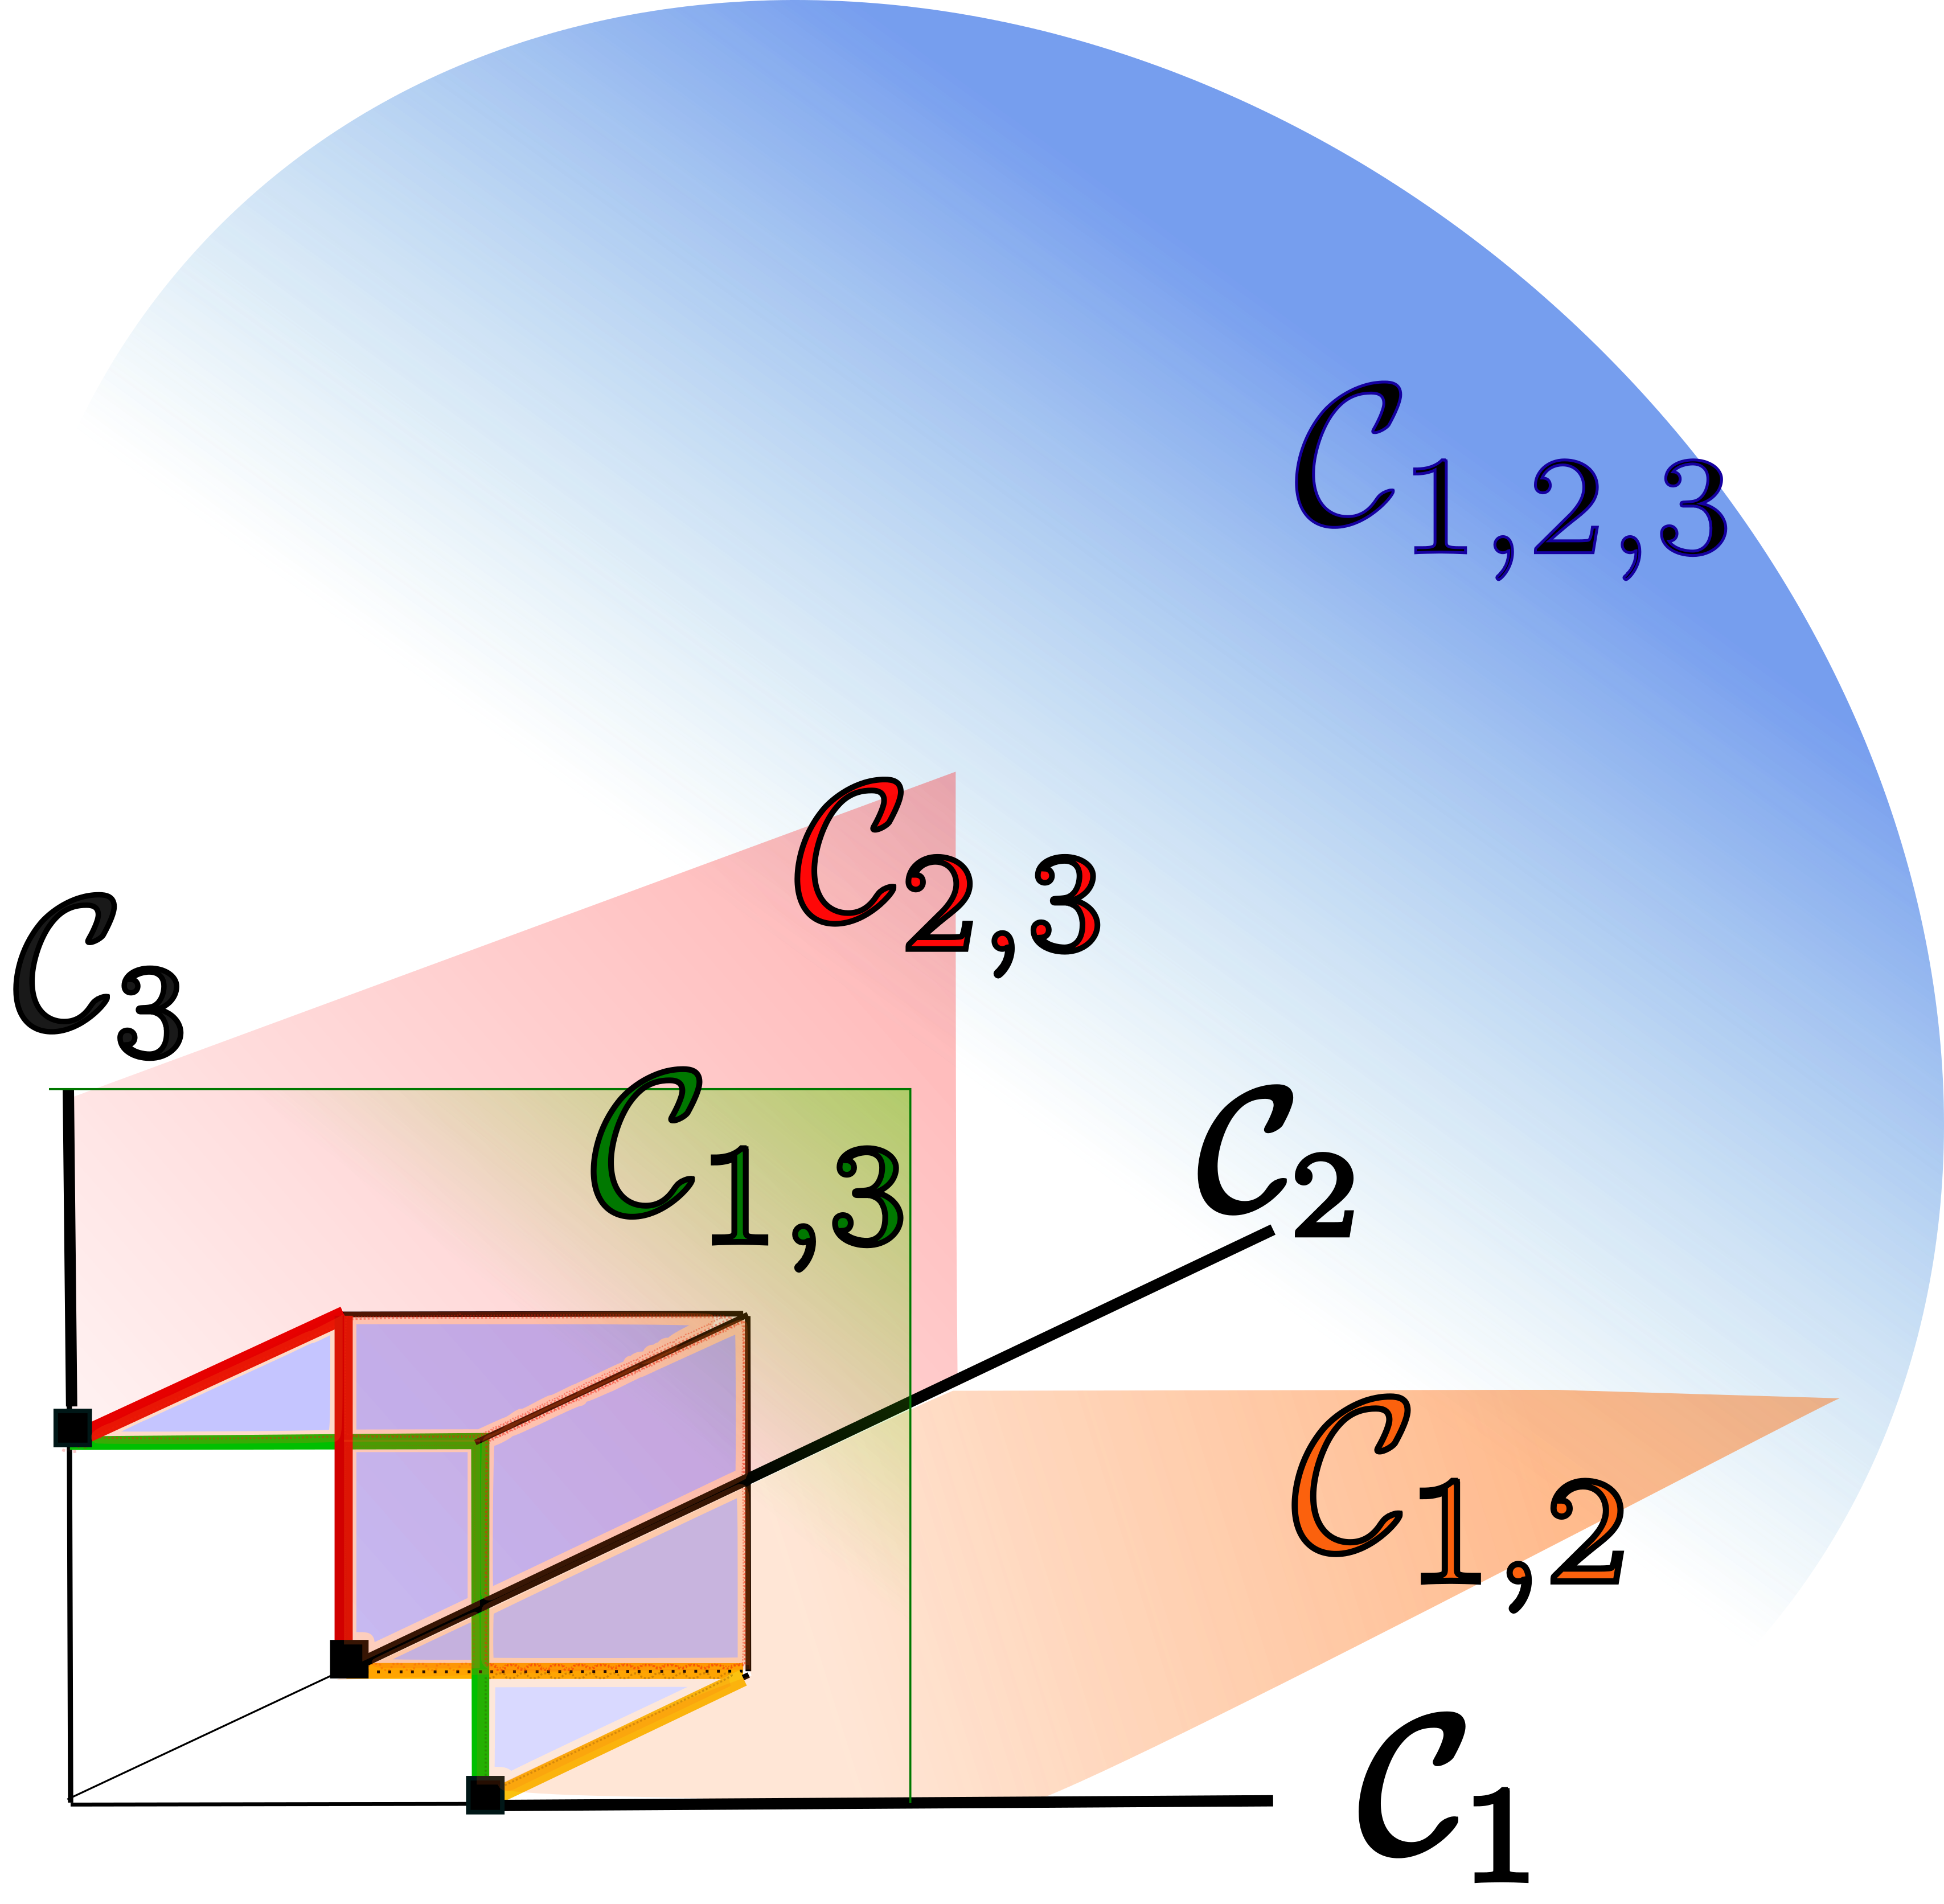
\includegraphics[scale=0.2]{fig_source/cone}
\captionof{figure}{Truncated cones in 3D}
\label{resume_fr:fig:3Dcones}
\end{minipage}\hfill
\begin{minipage}{0.5\linewidth}
\centering
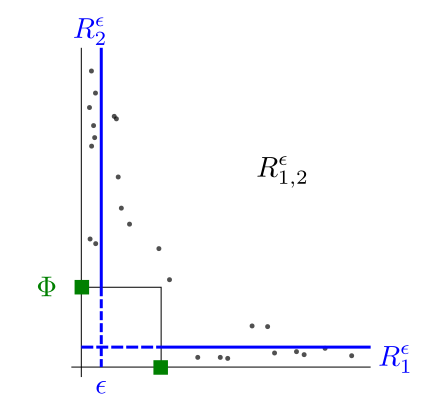
\includegraphics[width=0.64\linewidth]{fig_source/representation2D}
\captionof{figure}{Truncated $\epsilon$-cones in 2D}
\label{resume_fr:2Dcones}
\end{minipage}


This is done using $\epsilon$-thickened sub-cones $\cone_\alpha^\epsilon$, corresponding to $\epsilon$-thickened sub-spheres $\Omega_\alpha^\epsilon$, as shown in Figure~\ref{resume_fr:2Dcones} in the two-dimensional case.
We thus obtain an estimate $\widehat{\mathcal{M}}$ of the representation
$$\mathcal{M} = \{ \Phi(\Omega_{\alpha}):\; \emptyset \neq \alpha\subset\{1,\; \ldots,\; d \}\}.$$
Theoretically, recovering the $(2^{d}-1)$-dimensional unknown
vector $\mathcal{M}$ amounts to roughly approximating the support of $\Phi$ using the partition
$\{\Omega_\alpha, \alpha\subset\{1,\ldots,d\}, \alpha\neq \emptyset\}$, that is, determine which $\Omega_\alpha$'s have
nonzero mass (and evaluating the mass $\Phi(\Omega_\alpha)$), or equivalently, which $\Phi_\alpha$'s are nonzero. This support estimation is potentially
sparse (if a small number of $\Omega_\alpha$ have non-zero mass, \ie~Phenomenon~\textbf{1-}) and
potentially low-dimensional (if the dimensions of the sub-spheres $\Omega_\alpha$ with non-zero mass are low, \ie~Phenomenon~\textbf{2-}).

% Second, investigate how the angular measure $\Phi$ spreads its mass on the
% $\Omega_{\alpha}$'s, the theorical quantity $\Phi(\Omega_{\alpha})$ indicating to which extent extreme observations may occur in the `direction' $\alpha$ for $\emptyset \neq \alpha \subset \{1,\; \ldots,\; d \}$. 

% These two goals are achieved using empirical versions of
% the angular measure, evaluated on the $\epsilon$-thickened sub-spheres $\Omega_\alpha^\epsilon$.

\textbf{Anomaly Detection.}
Our proposed algorithm, DAMEX for Detecting Anomalies with Extremes, learns $\widehat{\mathcal{M}}$, a (possibly sparse and low-dimensional) representation of the angular measure, from which a scoring function can be defined in the context of anomaly detection.
The underlying assumption is that an observation is potentially abnormal if its `direction' (after a standardization of each marginal) is special regarding the other extreme observations. In other words, if it does not belong to the (sparse) representation $\widehat{\mathcal{M}}$. See Chapter~\ref{jmva} for details on how the scoring function is defined from this representation.
According to the benchmarks derived in this chapter, DAMEX significantly improves the performance (both in term of precision and of ROC curves) in extreme regions, inducing \eg~more vertical ROC curves near the origin.

\textbf{Theoretical grounds.}
From the work on the \stdf~estimation summarized in the previous sub-section~\ref{resume_fr:stdf}, in particular from Theorem~\ref{resume_fr:thm-princ} and from the ideas used to prove Theorem~\ref{resume_fr:thm:l}, we are able to derive some theoretical guaranties for this approach.
%
Under non-restrictive assumptions standard in EVT (existence of the angular measure and continuous marginal c.d.f.), we obtain a non-asymptotic bound of the form
\begin{align*}
\sup_{\emptyset \neq \alpha \subset \{1,\; \ldots,\; d \}}~ |\widehat{\mathcal{M}}(\alpha)- \mathcal{M}(\alpha)|
~\le~  C d \left( \sqrt{ \frac{1}{\epsilon k}\log\frac{d}{\delta}} + M d\epsilon \right) + \text{bias}(\epsilon, k, n),
\end{align*}
with probability greater than $1-\delta$, where $k = k(n) \to \infty$ with $k(n) = o(n)$ can be interpreted as the number of data considered as extreme. 
The bias term goes to zero as $n \to \infty$, for any fixed $\epsilon$.




\section{Heuristic approaches}
\label{resume_fr:sec:heuristic}

The two contributions in this section are of heuristic nature and not yet supported by statistically sound theoretical results. Although this ongoing work has not been published yet and will certainly be completed in the near future, we believe that it has its place in our manuscript, given the numerous convincing numerical experiments we carried out and the rationale behind the approaches promoted we gave.
%
These two contributions address two major challenges in anomaly detection:

\begin{itemize}
\item How to evaluate unsupervised anomaly detection in practice?
\item How to grow random forests with only one class available?
\end{itemize}

The first point has been partially addressed in Section~\ref{resume_fr:scoring} with MV and EM curves.
However, these two criteria have originally been introduced to build scoring functions \emph{via} Empirical Risk Minimization (ERM), and no study has been made on their use to evaluate scoring functions as ROC or PR criteria do.
Besides, their use to measure the quality of a scoring function $s_n$ involves the computation of the Lebesgue measure  $\leb(s_n \ge u)$, which is very challenging in high dimensional frameworks. 

The two proposed approaches are heuristic-based, and no theoretical guarantees such as consistency or convergence rates are derived. However, extensive benchmarks show the relevance of these approaches.

\subsection{Evaluation of anomaly detection algorithms}
\label{resume_fr:evaluation}
This is a summary of Chapter~\ref{chap:evaluation}, which is based on a workshop paper \citep{ICMLworkshop16} and a work to be submitted \citep{NIPS16evaluation}.


When sufficient labeled data are available, classical criteria based on ROC \citep{Provost1997, Provost1998, Fawcett2006} or PR \citep{Davis2006, Clemencon2009} curves can be used to compare the performance of unsupervised anomaly detection algorithms. However, in many situations, few or no data are labeled. This calls for alternative criteria one can compute on non-labeled data.

While excess-mass and mass-volume curves quantities have originally been introduced to build scoring functions \emph{via}
Empirical Risk Minimization (ERM), the MV-curve has been used recently for the calibration of the One-Class SVM \citep{Thomas2015}.
When used to attest the quality of some scoring function, the volumes induced become unknown and must be estimated, which is challenging in large dimension if no prior knowledge on the form of these level sets is available.
%
Besides, the accuracy of EM or MV curves as evaluation criteria has not been studied yet.
%
Summarized in this section and as a contribution of this thesis, numerical performance scores based on EM and MV criteria (that do not require labels) are empirically shown to discriminate accurately (\wrt~ROC or PR based criteria) between algorithms.
%These criteria are based on existing Excess-Mass (EM) and Mass-Volume (MV) curves, which generally cannot be well estimated in large dimension.
A methodology based on feature sub-sampling and aggregating is also described and tested. This extends the use of these criteria to high-dimensional datasets and solves major drawbacks inherent to standard EM and MV curves.

Recall that the MV and EM curves of a scoring function $s$ can be written as
\noindent
\begin{align}
\label{resume_fr:intro:MV-def}
 MV_s(\alpha) &= \inf_{u \ge 0}~~ \leb(s \ge u) ~~\st~~\mathbb{P}(s(\mb X) \ge u) \ge \alpha\\
\label{resume_fr:intro:EM-def}
 EM_s(t) &= \sup_{u \ge 0}~~ \mathbb{P}(s(\mb X) \ge u) ~-~ t \leb(s \ge u)
\end{align}
for any $\alpha\in (0,1)$ and $t >0$.
%
The optimal curves are $MV^* = MV_f = MV_{T \circ f}$ and $EM^* = EM_f = EM_{T \circ f}$ for any increasing transform $T: \text{Im(f)} \to \mathbb{R}$.
%
As curves cannot be trivially compared, consider the $L^1$-norm $\|.\|_{L^1(I)}$ with $I\subset \rset$ an interval. As $MV^*=MV_f$ is below $MV_s$ pointwise, $\argmin_s \| MV_s - MV^* \|_{L^1(I)} = \argmin \| MV_s \|_{L^1(I)} $. We thus define
$\crit^{MV}(s) = \| MV_s \|_{L^1(I^{MV})},$ which is equivalent to consider $\| MV_s - MV^* \|_{L^1(I^{MV})}$ as mentioned in the introduction. As we are interested in evaluating accuracy on large density level-sets, one natural interval $I^{MV}$ would be for instance $[0.9, 1]$. However, MV diverges in $1$ when the support is infinite, so that we arbitrarily take $I^{MV} = [0.9, 0.999].$
The smaller is $\crit^{MV}(s)$, the better is the scoring function $s$.
%
Similarly, we consider $\crit^{EM}(s) = \| EM_s \|_{L^1(I^{EM})}, $ this time with $I^{EM} = [0,EM^{-1}(0.9)],$ where $EM_s^{-1}(0.9) := \inf\{t\ge 0,~ EM_s(t) \le 0.9\}$, as $EM_s(0)$ is finite (equal to $1$). % We point out that such small values of $t$ correspond to large level-sets. Also in practice, we have observed that
% $EM_s^{-1}(0.9)$ (as well as $EM_f^{-1}(0.9)$) varies significantly depending on the dataset. Generally, for datasets in large dimension, it can be % $\widehat{EM}_s^{-1}(0.9)$ is
% very small (in the experiments, smallest values are of order $10^{-7}$) as it is of the same order of magnitude as the inverse of the total support volume.

As the distribution $F$ of the normal data is generally unknown, MV and EM curves must be estimated. Let $s\in \mathcal{S}$ and $\mb X_1,\; \ldots,\; \mb X_n$ be an i.i.d. sample with common distribution $F$ and set $\mathbb{P}_n(s \ge t)=\frac{1}{n}\sum_{i=1}^n\mathds{1}_{s(\mb X_i)\geq t}.$ The empirical MV and EM curves of $s$ are then simply defined as empirical version of \eqref{resume_fr:intro:MV-def} and \eqref{resume_fr:intro:EM-def}, 
\begin{align}
\label{resume_fr:MV-def-emp}
\widehat{MV}_s(\alpha) = \inf_{u \ge 0} \left\{ \leb(s \ge u) ~~\st~ \mathbb{P}_n(s \ge u) \ge \alpha \right\}
\end{align}
\begin{align}
\label{resume_fr:EM-def-emp}
\widehat{EM}_s(t) = \sup_{u \ge 0} \mathbb{P}_n(s \ge u) ~-~ t \leb(s \ge u)
%\lambda_s \circ \alpha_s^{-1}(\alpha),
\end{align}
%
%
Finally, we obtain the empirical EM and MV based performance criteria:
\begin{align}
\label{resume_fr:eq:standard_emp_EM}\widehat{\crit}^{EM}(s) &= \| \widehat{EM}_s \|_{L^1(I^{EM})}  &&I^{EM} = [0,\widehat{EM}^{-1}(0.9)],\\
\label{resume_fr:eq:standard_emp_MV}\widehat{\crit}^{MV}(s) &= \| \widehat{MV}_s \|_{L^1(I^{MV})}  &&I^{MV} = [0.9, 0.999].
\end{align}
%
% As the distribution $F$ is generally unknown, excess-mass curves must be estimated. Let $s\in \S$ and $\mb X_1,\; \ldots,\; \mb X_n$ be an i.i.d. sample with common distribution $F$ and set $$\widehat{\alpha}_s(t)=(1/n)\sum_{i=1}^n\mathds{1}_{s(X_i)\geq t}.$$ The empirical $EM$ curve of $s$ is then defined as $$\widehat{EM}_s(t)=\sup_{u>0}\{ \widehat{\alpha}_s(u)-t\lambda_s(u)\}.$$ In practice, just as with the mass-volume criterion (drawback \textbf{1}), it may be difficult to estimate the volume $\lambda_s(u)$ and Monte-Carlo approximation can naturally be used for this purpose.

% Note that in practice, the volume $\leb(s \ge u)$ is estimated using Monte-Carlo approximation, which only applies to small dimensions.
% %
% This is a major drawback for the use of excess-mass or mass-volume criteria in high dimensional framework, if no prior knowledge on the form of these level sets is available. Besides, there has been no work yet dealing with EM or MV curves as evaluation criteria, as they have originally been introduced to build scoring scoring function via ERM.
%
The methodology to scale the use of the EM and MV criteria to large dimensional data consists in sub-sampling training \emph{and} testing data along features, thanks to a parameter $d'$ controlling the number of features randomly chosen for computing the (EM or MV) score. Replacement is done after each draw of features $F_1,\ldots,F_{m}$. A partial score $\widehat \crit_k^{MV}$ (resp. $\widehat \crit_k^{EM}$) is computed for each draw $F_k$ using \eqref{resume_fr:eq:standard_emp_EM} (resp. \eqref{resume_fr:eq:standard_emp_MV}). The final performance criteria are obtained by averaging these partial criteria along the different draws of features. This methodology is described in Algorithm~\ref{resume_fr:algo:EMMV}.
%
\begin{algorithm}[!tbh]
\caption{~~High-dimensional EM/MV: evaluate AD algorithms on high-dimensional data}
\label{resume_fr:algo:EMMV}
\begin{algorithmic}
  \STATE \textbf{Inputs}: AD algorithm $\mathcal{A}$, data set $X = (x^j_i)_{1 \le i \le n, 1 \le j \le d }$, feature sub-sampling size $d'$, number of draws $m$.
  \FOR{$k=1,\ldots,m$}
    \STATE{randomly select a sub-group $F_k$ of $d'$ features}
    \STATE{compute the associated scoring function $\widehat s_{k} = \mathcal{A}\big((x^j_i)_{1 \le i \le n,~j \in F_k}\big)$}
    \STATE compute $\widehat{\crit}_k^{EM} = \| \widehat{EM}_{\widehat s_k} \|_{L^1(I^{EM})}$ using \eqref{resume_fr:eq:standard_emp_EM} or $\widehat{\crit}_k^{MV} = \| \widehat{MV}_{\widehat s_k} \|_{L^1(I^{MV})}$ using \eqref{resume_fr:eq:standard_emp_MV}
  \ENDFOR 
  \STATE \textbf{Return} performance criteria: $$\widehat{\crit}^{EM}_{high\_dim} (\mathcal{A})= \frac{1}{m} \sum_{k=1}^m\widehat \crit_k^{EM} \text{~~~~(idem for MV)}$$
\end{algorithmic}
\end{algorithm}

Low-dimensional and high-dimensional EM/MV are tested \wrt~three classical AD algorithms. A wide range on real labeled datasets are used in the benchmark.
Experiments show that when one algorithm has % \emph{clearly} (according to both EM and PR scores)
better performance than another on some fixed dataset, according to both ROC and PR AUCs, one can expect to recover it without using labels with an accuracy of $82\%$ in the novelty detection framework, and $77\%$ in the unsupervised framework.


\subsection{One-Class Random Forests}
\label{resume_fr:ocrf}
This is a summary of Chapter~\ref{chap:ocrf}, which is based on work \citep{OCRF16} to be submitted.

%Scoring functions built by optimizing EM or MV criteria usually not perform well. 

Building accurate scoring functions by optimizing EM or MV criteria is very challenging in practice, just as building classifiers by optimizing the ROC curve (\cite{Clemencon2010}) in the supervised framework.
%
More work is needed for these methods to be efficient in practice, particularly for the choice of the class of sets on which the optimization is done.
%
Indeed, % optimization is done over some class of scoring functions
this class is \emph{hopefully rich enough to provide a good approximation while simple enough to control the convergence rate}. This compromise is hard to achieve, especially in high dimension when no prior knowledge on the shape of the level sets is available. 
%
% In addition, if criterion optimization is useful when no intuition is available on the underlying problem, this is not the case in anomaly detection. We usually do not try to minimize ROC curves to have a good classifier, and a doctor usually does not health people by trying to optimize tensiometer or stethoscope measurements. 
%
% To derive guaranties of theoretical nature (namely to attest the relevance of the algorithm in terms of \eg~ROC or EM/MV criteria), optimizing these evaluation criteria is often an efficient way. 
% But this does not remains true in terms of empirical performance. 
In this section, we propose a heuristic approach to build scoring functions using Random Forests (RFs) \citep{Breiman2001, Genuer2008, Biau2008, Biau2016}. % , which are an intuitive way of performing classification and regression.
More formally, we adapt RFs to the one-class classification framework by introducing one-class splitting criteria.

Standard RFs are estimators that fit a number of decision tree
classifiers on different random sub-samples of the dataset.
Each tree is built recursively, according to a splitting criterion based on
some impurity measure of a node. The prediction is done by an average over each tree prediction. In classification the averaging is based on a majority vote.
Few attempts to transfer the idea of RFs to one-class
classification have already been made \citep{Desir12, Liu2008, Shi2012}.
%, Clemencon2014}. On ne cite pas clemencon2014 car leur algorythm treeRank n'est pas des RFs (base estimator = non-symetric ranking trees) (en fait unsupervisedTreeRank c'est juste une modif triviale de TreeRank en considerant des volumes)
%
No algorithm structurally extends (without second class sampling and without alternative base estimators) RFs to one-class classification.

We introduce precisely such a methodology. It builds on a natural adaptation of two-class % Gini improvement proxy, yielding a one-class Gini-based criterion specially designed for
splitting criteria to the one-class setting, as well as an adaptation of the two-class majority vote.
In addition, it turns out that the one-class model promoted here corresponds to the asymptotic behavior of an adaptive (with respect to the tree growing process) outliers generating methodology.

\textbf{One-class Model with parameters ($n$, $\boldsymbol{\alpha}$).}
We consider a random variable $ X:\Omega \to \mathbb{R}^d$ \wrt~a probability space $(\Omega, \mathcal{F}, \mathbb{P})$.
The law of $X$ depends on another \rv~$y \in \{0,1\}$, verifying $\mathbb{P}(y=1)=1-\mathbb{P}(y=0)=\alpha$. We assume that conditionally on $y=0$, $ X$ follows a law $F$, and conditionally on $y=1$ a law $G$:
\begin{align*}
 X ~|~ y=0 ~~\sim~~ F, &~~~~~~~~~~  \mathbb{P}(y=0)=1-\alpha, \\
 X ~|~ y=1 ~~\sim~~ G, &~~~~~~~~~~  \mathbb{P}(y=1)=\alpha.
\end{align*}
%
We model the one-class framework as follows. Among the $n$ \iid~observations, we only observe those with $y=0$ (the normal behavior), namely $N$ realizations of $( X ~|~ y=0)$, where $N$ is itself a realization of a \rv~$\mb N$ of law $\mb N \sim \text{Bin}\big(n, (1-\alpha)\big)$, the binomial distribution with parameters $(n, p)$. As outliers are not observed, we classically assume that $G$ follows a uniform distribution on the hyper-rectangle $\mathcal{X}$ containing all the observations, so that $G$ has a constant density $g(x) \equiv 1 / \leb(\mathcal{X})$ on $\mathcal{X}$. This assumption \emph{will be removed} in the adaptive approach, where no prior distribution is assumed for the outliers.
%laisser une ligne car fin du model one class

One-class empirical analogues of two-class impurity measures are then obtained by replacing the quantities relative to the normal behavior by their empirical versions.
The quantities relative to the unobserved second class (abnormal behavior) are naturally expressed using the uniform distribution assumption.

In this way, our one-class impurity improvement function corresponds to the two-class one, where empirical second class quantities have been replaced by their expectation assuming a uniform distribution.

But it also induces a major problem: those expectations, which are proportional to the volume of the node at stake, become very small when going deeper in the tree. In the two-class framework, the corresponding problem is when the second class is highly under-represented in the neighborhood of the observations. 
%
As we assume the second class to be uniform on a hyper-rectangle containing all the observations, this fact was expected, especially in large dimension (curse of dimensionality). 
%
As the quantities relative to the second class are very close to zero, one observes that the impurity criterion becomes constant when the split varies, and then useless.

\textbf{Adaptive approach.}
%
A solution is to chose adaptively (\wrt~the volume of each node) the number $\alpha n$, which can be interpreted as the number of (hidden) outliers. Recall that neither $n$ nor $\alpha$ is observed in One-Class-Model($n$, $\alpha$) defined above. 

The idea is to make $\alpha(t) \to 1$, $n(t) \to \infty$ when the volume of node $t$ goes to zero.
%
In other words, instead of considering one fixed general model One-Class-Model($n$, $\alpha$), we adapt it to each node $t$, considering One-Class-Model($n(t)$, $\alpha(t)$) \emph{before searching the best split}. We still consider the $N$ normal observations as a realization of this model. When growing the tree, using One-Class-Model($n(t)$, $\alpha(t)$) allows to maintain a non-negligible expected proportion of outliers in the node to be split, even when its volume becomes close to zero.
Of course, constraints have to be made to ensure consistency between all these models.
%
For instance, recalling that the number $N$ of normal observations is a realization of $\mb N$ following a Binomial distribution with parameters $(n, 1-\alpha)$, a first natural constraint on $\big(n(t), \alpha(t)\big)$ is
\begin{align}
\label{resume_fr:constraint1}
(1-\alpha)n = \big(1-\alpha(t)\big) \cdot n(t) \text{~~~~~for all~~} t,
\end{align}
so that the expectation of $\mb N$ remains unchanged. 
Then the asymptotic model (when the volume of $t$ goes to $0$) consists in fact in assuming that the number $N$ of normal data we observed is a realization of a Poisson distribution $\mathcal{P}\big((1-\alpha)n\big)$, and that an infinite number of outliers have been hidden. In the two class framework, this corresponds to observing an infinite number of outliers distributed closely around, outside and inside the support of the normal distribution, breaking the curse of dimensionality when using uniformly distributed outliers (see Chapter~\ref{chap:ocrf} for details).

\begin{remarque}[\textbf{Basic idea behind the adaptive approach}]
This work corresponds in fact to the following simple idea that allows us to split a node without examples of the second class.
Each time we are looking for the best split for a node $t$, we simply replace (in the 2-class impurity decrease to be maximized) the second class proportion in the left node $t_L$ by the proportion expectation $volume(t_L)/volume(t)$ (idem for the right node).
It ensures that one child node tries to capture the maximum number of observations with a minimal volume, while the other child looks for the opposite. %Such volume constraint/mass objective are similarly used to define minimum-volume sets.
\end{remarque}


\begin{remarque}[\textbf{No sampling}]
The corresponding sampling method is the following: for each note $t$ to be splitted containing $n_t$ observations (inliers), generate $n_t$ uniform outliers over the corresponding cell to optimize a two-class splitting criterion. We precisely \emph{avoid sampling} the outliers by using the proportion expectation $volume(t_L)/volume(t)$.
\end{remarque}



\textbf{One-Class RF algorithm.} Let us summarize the algorithm in its most generic version.
It has $7$ parameters:
$max\_samples$, $max\_features\_tree$, $max\_features\_node$, $\gamma$, $max\_depth$, $n\_trees$, $s_k$.
%
Each tree is classically grown on a random subset of both the input samples and the input features \citep{Ho1998, Panov2007}.
This random subset is a sub-sample of size $max\_samples$, with $max\_features\_tree$ variables chosen at random without replacement (replacement is only done after the tree is grown). The tree is built by minimizing 
a one-class version of the Gini criterion \citep{Gini1912}, obtained by replacing empirical quantities related to the (unobserved) second class by population ones. These correspond to a weighted uniform distribution, the weight increasing when the volume of the node decreases, in order to avoid highly unbalanced classes (volume vs. observations). Indeed when their depth increases, the nodes tend to have smaller volumes while keeping as much (normal) observations as they can.

New nodes are built (by minimizing this criterion) until the maximal depth $max\_depth$ is achieved.
% define a large number of geometric features and search over a random selection
% of these for the best split at each node
% In addition, this is done
Minimization is done as introduced in \citep{Amit1997}, by defining a large number $max\_features\_node$ of geometric features and searching over a random selection of these for the best split at each node.
%
The forest is composed of a number $n\_trees$ of trees. The predicted score of a point $x$ is given by $s_k(x)$, which is either the stepwise density estimate (induced by the forest) around $x$, the local density of a typical cell containing $x$ or the averaged depth of $x$ among the forest. Chapter~\ref{chap:ocrf} formally defines the one-class splitting criteria and provides an extensive benchmark of state-of-the-art anomaly detection algorithms.








\section{Scikit-learn contributions}
\label{resume_fr:sec:impl}

As an other contribution of this thesis, two classical anomaly detection algorithms, Isolation Forest and Local Outlier Factor have been implemented and merged on scikit-learn. These algorithms are presented in the Background Part, Section~\ref{sec:AD_sklearn}. % on Anomaly Detection in Scikit-Learn. 

Scikit-learn, see \cite{sklearn2011}, is an open-source library providing well-established machine learning methods.
It is a Python module, the latter language being very popular for scientific computing, thanks to its high-level interactive nature. % Python is enjoying this recent years a strong expansion both in academic and industrial settings. Scikit-learn takes advantage of this favourable backdrop and extends this general-purpose programming language with machine learning operation: 
Scikit-learn provides a composition mechanism (through a \emph{Pipeline} object) to combine estimators, preprocessing tools and model selection methods in such a way the user can easily construct complex ad-hoc algorithms.
%
The development is done on \emph{Github}\footnote{https://github.com/scikit-learn}, a Git repository hosting service which facilitates collaboration, as coding is done in strong interaction with other developers. Because of the large number of developers, emphasis is put on keeping the project maintainable, \eg~by avoiding duplicating code at the price of a reasonable loss of computational performance.%up to pay (reasonably) in computational performance. 


This contribution was supervised by Alexandre Gramfort and was funded by the Paris Saclay Center for Data Science. It also includes work for the scikit-learn maintenance like resolving issues and reviewing other contributors' pull requests.

% XXX: add contribution with A.Muller


\section{Conclusion and Scientific Output}
\label{resume_fr:intro:concl}
The contributions of this thesis can be summarized as follows. 

First, an adequate performance criterion called Excess-Mass curve is proposed (Section~\ref{resume_fr:em-curve}), in order to compare possible candidate scoring function and to pick one eventually. 
The corresponding publication is \cite{AISTAT15}:
\begin{itemize}
\item On Anomaly Ranking and Excess-Mass Curves. (AISTATS 2015).\\
Authors: Goix, Sabourin, and Clémençon. 
\end{itemize}

% This is a major drawback for its use in high dimensional framework, if no prior knowledge on the form of these level sets is available. 


%However, to measure with this criterion the quality of a scoring function $s_n$, volume of level sets of $s_n$ have to be compute which is a considerable drawback for its use in high dimensional framework, if no prior knowledge on the form of these level sets is available.

As a second contribution, we bring advances in multivariate EVT by providing non-asymptotic bounds for the estimation of the STDF, a functional characterizing the extreme dependence structure (Section~\ref{resume_fr:stdf}). The corresponding publication is \cite{COLT15}:
\begin{itemize}
\item Learning the dependence structure of rare events: a non-asymptotic study. (COLT 2015).\\
Authors: Goix, Sabourin, and Clémençon.
\end{itemize}

The third contribution is to design a statistical method that produces a (possibly sparse) representation of the dependence structure of extremes, while deriving non-asymptotic bounds to assess the accuracy of the estimation procedure (Section~\ref{resume_fr:sec:JMVA}).
%
This contribution also includes a multivariate EVT-based algorithm which returns a scoring functions defined in extreme regions. This directly applies to anomaly detection as an abnormality score.
The corresponding publications are \cite{AISTAT16}, \cite{NIPSWORKSHOP15} and \cite{ARXIV16}:
%
\begin{itemize}
\item Sparse Representation of Multivariate Extremes with Applications to Anomaly Ranking. (AISTATS 2016 and NIPS 2015 Workshop on Nonparametric Methods for Large Scale Representation Learning).\\
Authors: Goix, Sabourin, and Clémençon.
\item Sparse Representation of Multivariate Extremes with Applications to Anomaly Detection. (Under review for Journal of Multivariate Analysis).\\
Authors: Goix, Sabourin, and Clémençon.
\end{itemize}





As a fourth contribution, we show (empirically) that EM or MV based criteria are able to discriminate accurately (\wrt~ROC or PR based criteria) between scoring functions in low dimension. Besides, we propose a methodology based on feature sub-sampling and aggregating to scale the use of EM or MV to higher dimensions.
The corresponding publications are \cite{ICMLworkshop16} and \cite{NIPS16evaluation}:
\begin{itemize}
\item How to Evaluate the Quality of Unsupervised Anomaly Detection Algorithms? (ICML 2016, Workshop on Anomaly Detection). % Co-winner of the Best Paper Award, sponsored by Google.
  \\
Author: Goix. 
\item How to Evaluate the Quality of Unsupervised Anomaly Detection Algorithms? (to be submitted).\\ Authors: Goix and Thomas. 
\end{itemize}


The fifth contribution of this thesis is to develop an efficient heuristic for building accurate scoring functions. This is done by generalizing random forests to one-class classification. The corresponding work (to be submitted) is \cite{OCRF16}: 
\begin{itemize}
\item One-Class Splitting Criteria for Random Forests with Application to Anomaly Detection. (to be submitted).\\
Authors: Goix, Brault, Drougard and Chiapino.
\end{itemize}



As a last contribution, two classical anomaly detection algorithms have been implemented and merged on scikit-learn. They are used in this dissertation for empirical comparison purpose to attest the relevance of the forementionned approaches.
The pull requests of these two contributions are available here:
\begin{itemize}
\item https://github.com/scikit-learn/scikit-learn/pull/4163  (Isolation Forest)
\item https://github.com/scikit-learn/scikit-learn/pull/5279 (LOF)
\end{itemize}


% Eventually, we would like to notice that there still seems to be a significant gap to fill between theory and practice in anomaly detection. Trying to derive an algorithm supported by a theoretical analysis often affects the algorithm construction in such a way that it limits its efficiency in practice.
% On the opposite side, when trying to develop an algorithm which performs well in practice before thinking about any theoretical guaranties, it is often difficult to derive a statistical analysis. In this thesis, contributions have been made on both of these sides. Besides, the contribution on the sparse representation of multivariate extreme belongs to both theoretical and practical sides: it can be viewed as an efficient heuristic supported by a mathematical analysis from the extreme value theory, as well as an algorithm designed by this theory which can compete with state-of-the-art anomaly detection algorithms.


\paragraph{Context of this work.}
This thesis was carried out in the STA (Statistiques et Applications) team of the Signal and Image Processing (TSI) department at Telecom ParisTech. The contributions presented in this thesis were supported by Ecole Normale Supérieure de Cachan via a `contrat doctoral pour normalien' and by the industrial chair `Machine Learning for Big Data' from Telecom ParisTech. The scikit-learn contributions have been supported by the Paris Saclay Center for Data Science regarding the collaboration with Alexandre Gramfort, and by the forementioned machine learning chair as regards the collaboration at New York University with Andreas Müller.

\paragraph{Outline of the thesis.}
This dissertation is organized as follows. 
\begin{itemize}
\item Part~\ref{part:background} gathers the background work relevant to this thesis:

Chapter~\ref{chap:back_concentration} presents general results on measure concentration inequalities; 

Chapter~\ref{back:EVT} provides a concise background on extreme value theory;

Chapter~\ref{back:AD_scikit} reviews classical anomaly detection algorithms used in the benchmarks and provides illustrative examples with the scikit-learn library. It also presents relating code contributions.

\item Part~\ref{part:struct} deals with theoretical performance criteria for the anomaly ranking task:

Chapter~\ref{aistat:chap} presents the details on anomaly ranking and excess-mass curve, as summarized above Section~\ref{resume_fr:scoring}; %The corresponding published work is \cite{AISTAT15}.

\item Part~\ref{part:vect} focuses on EVT-based methods for anomaly detection:

Chapter~\ref{colt} deals with the stable tail dependence function as summarized above in Section~\ref{resume_fr:stdf}; %The corresponding publication is \cite{COLT15};

Chapter~\ref{jmva} describes how scoring functions can be build using EVT, as previously summarized in Section~\ref{resume_fr:sec:JMVA}.
%The corresponding publications are \cite{NIPSWORKSHOP15}, \cite{AISTAT16} and submitted work \cite{ARXIV16}.


\item Part~\ref{part:heuristic} gathers two efficient heuristic-based methodologies:

Chapter~\ref{chap:evaluation} deals with the evaluation of anomaly detection algorithms, as summarized above Section~\ref{resume_fr:evaluation}; %Chapter~\ref{resume:evaluation}.
%The corresponding publications are \cite{ICMLworkshop16} and \cite{NIPS16evaluation}.

Chapter~\ref{chap:ocrf} presents the details % on one class splitting criteria 
  (summarized above Section~\ref{resume_fr:ocrf}) on one-class random forests.
%The corresponding submitted work is \citep{OCRF16};


\end{itemize}
